\documentclass[10pt,a4paper]{article}
\usepackage[margin=20mm]{geometry}
\usepackage[T1]{fontenc}
\usepackage{lmodern,amsmath,amssymb,booktabs,longtable,graphicx,array,xcolor,hyperref,float}
\definecolor{navy}{RGB}{24,61,91}
\hypersetup{colorlinks=true,urlcolor=navy,linkcolor=navy,pdftitle={A063 v0.2.1 - Hicks invariant-surface qualification}}
\setlength{\parindent}{0pt}\setlength{\parskip}{5pt}
\begin{document}
{\Large\bfseries A063 v0.2.1 --- Hicks invariant-surface qualification}\par
{\small \textit{Analytical reference (selected T34 target); parent v0.2.0 preserved; no v1.0.7 certification.}}\par
\hrule\smallskip
\textbf{New gates: 7 PASS / 2 FAIL / 3 UNRESOLVED.}
\section*{Scientific question and preregistered hypotheses}
Does the closed $T(3,4)$ Beltrami vortex-line orbit admit a finite smooth stationary material/vorticity surface whose \emph{solid-torus core} is also knotted, and can this be certified as nonlinearly stable under coupled perturbed 3D Euler evolution? We contrast two constructions: (i) the previously failed constant-radius tube centered on the knot and (ii) regular stationary Hicks level sets $\psi=\psi_0$. The latter are not assumed to be knotted tubes.
\begin{align}
\psi(s,z)&=A\big[J(\lambda r/a)-(r/a)^2J(\lambda)\big]s^2/r^2,\\
J(x)&=\frac{\sin x}{x}-\cos x,\quad r=\sqrt{s^2+z^2},\quad\lambda=4.4934094579,\\
u_s&=-\frac{1}{s}\partial_z\psi,\quad u_z=\frac1s\partial_s\psi,\quad
u_\phi=\frac{\lambda\psi}{as},\quad\boldsymbol\omega=(\lambda/a)\mathbf u.
\end{align}
Therefore $\mathbf u\cdot\nabla\psi=0$ and $\boldsymbol\omega\cdot\nabla\psi=0$ for the exact first-Beltrami Hicks branch, wherever $\nabla\psi\ne0$. We independently evaluate numerical normals using centered derivatives of analytic $\psi$ against the separately evaluated analytic velocity.
\section*{1. Explicit regular level surfaces}
The vortex-line initial position $s_0/a=0.9683098302$, and its reconstructed level is $\psi_0=0.138575114976$. We solve $\psi(s_c+r(\theta)\cos\theta,r(\theta)\sin\theta)=q\psi_0$ for $q\in\{0.9,1,1.1\}$, with 96, 192 and 384 meridional samples. The radial solutions are single-valued and strictly positive in the tested intervals. Revolving each curve around the symmetry axis yields a regular embedded torus.
\begin{table}[H]\centering\small\begin{tabular}{rrrrr}\toprule
$\psi/\psi_0$ & $s_{\min}/a$ & sphere clearance $/a$ & $W$ & max $|u_n|/u_{\rm rms}$ \\
\midrule
0.90 & 0.13882 & 0.02850 & 0.747563717 & 5.909e-08 \\
1.00 & 0.14666 & 0.03169 & 0.750000000 & 5.900e-08 \\
1.10 & 0.15418 & 0.03488 & 0.752329435 & 5.887e-08 \\
\bottomrule\end{tabular}\end{table}
\begin{figure}[H]\centering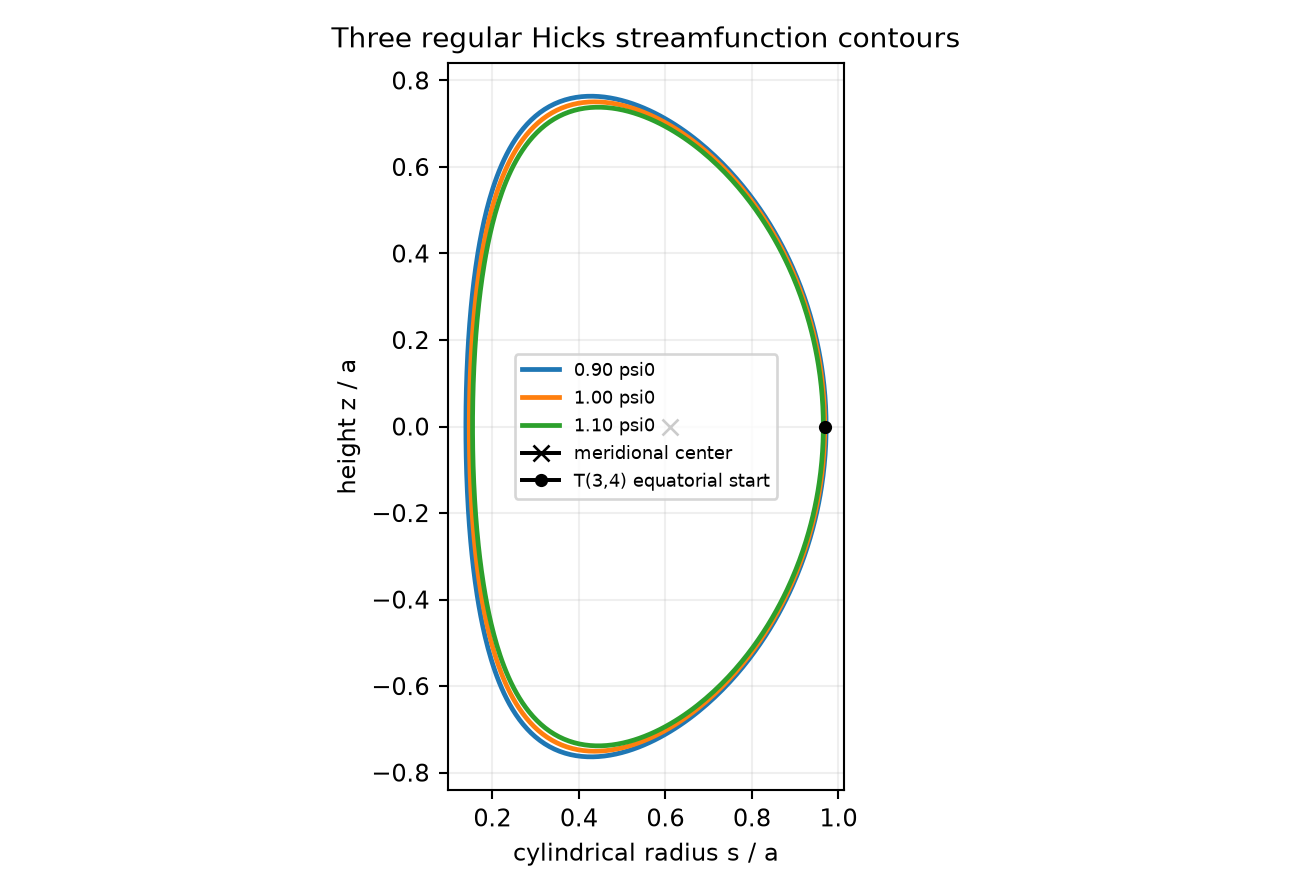
\includegraphics[width=.69\linewidth]{psi_meridional_levels.png}\caption{Closed nested meridional $\psi$ contours. Each avoids the axis $s=0$ and the sphere boundary.}\end{figure}
\section*{2. Topology: unknotted invariant torus, knotted line ON the torus}
The meridional contours are star-shaped about $s=s_c,z=0$, and can be continuously deformed to a small circle by $r_t(\theta)=(1-t)r(\theta)+tr_*$ without touching $s=0$. Revolution constructs an explicit isotopy to the \textbf{standard, unknotted solid torus}. Its core is a planar circle $C(\phi)=(s_c\cos\phi,s_c\sin\phi,0)$, an unknot. In contrast, the original $T(3,4)$ trajectory winds three times azimuthally and four times meridionally on the \emph{boundary} $\psi=\psi_0$. The torus is not a knotted tubular neighborhood whose solid-torus core is $T(3,4)$.
\begin{figure}[H]\centering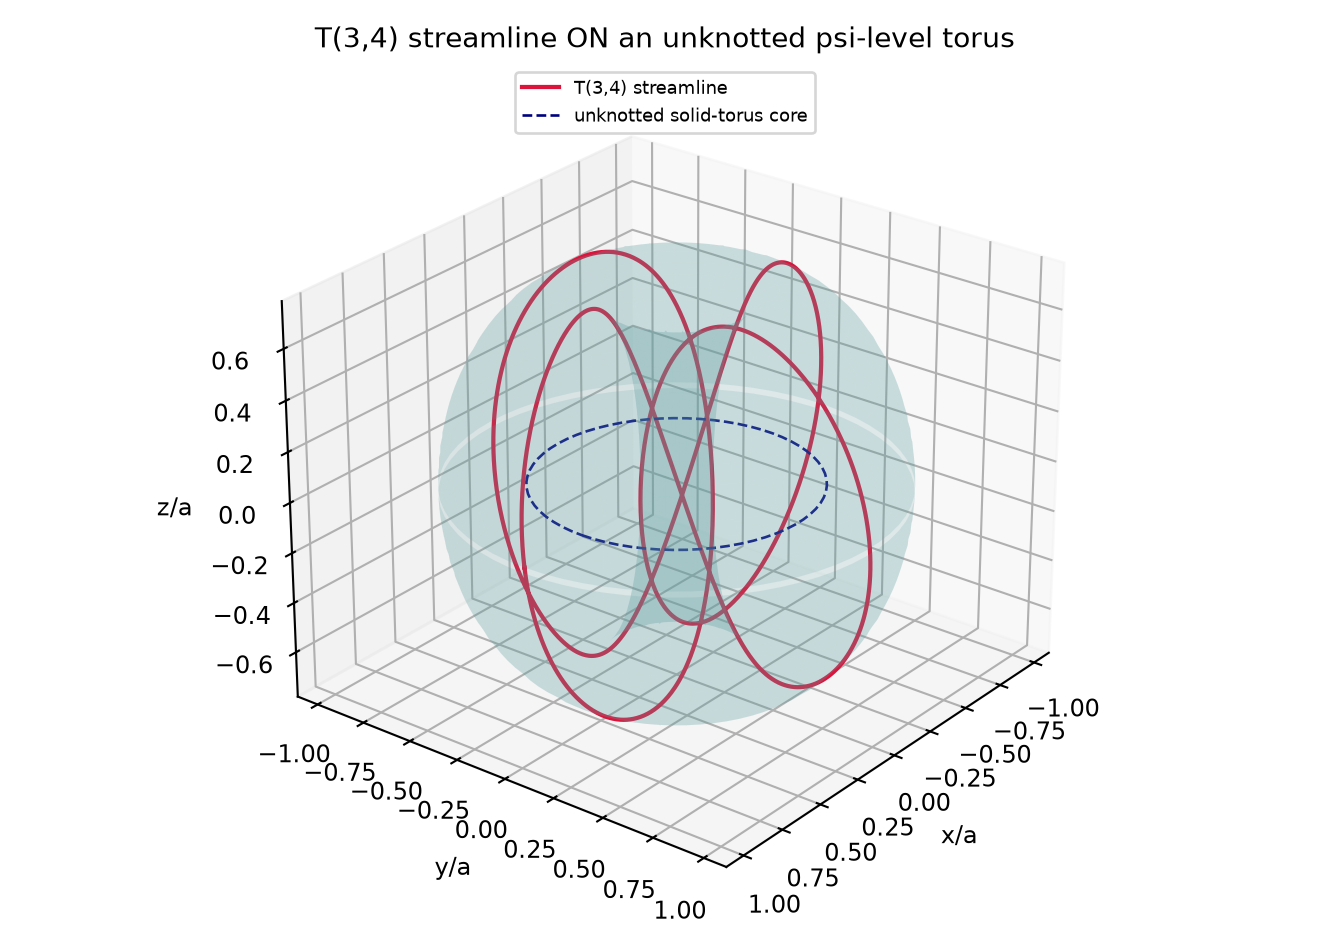
\includegraphics[width=.73\linewidth]{unknotted_psi_torus_T34.png}\caption{An invariant standard torus (translucent), the red knotted vortex line, and the dashed unknotted circle that is the solid-torus core.}\end{figure}
\section*{3. Material and vorticity flux}
The exact invariant surface has zero normal flux. A separate numerical check yields the normal-velocity values above; Richardson-like reduction across finite-difference steps checks convergence to zero. Since $\omega=(\lambda/a)u$, the exact vorticity-normal flux is zero too. This is \textbf{not} a localized vortex tube: the volume enclosed is a standard solid torus and the original Hicks flow has distributed vorticity throughout the spherical vortex aggregate.
\begin{figure}[H]\centering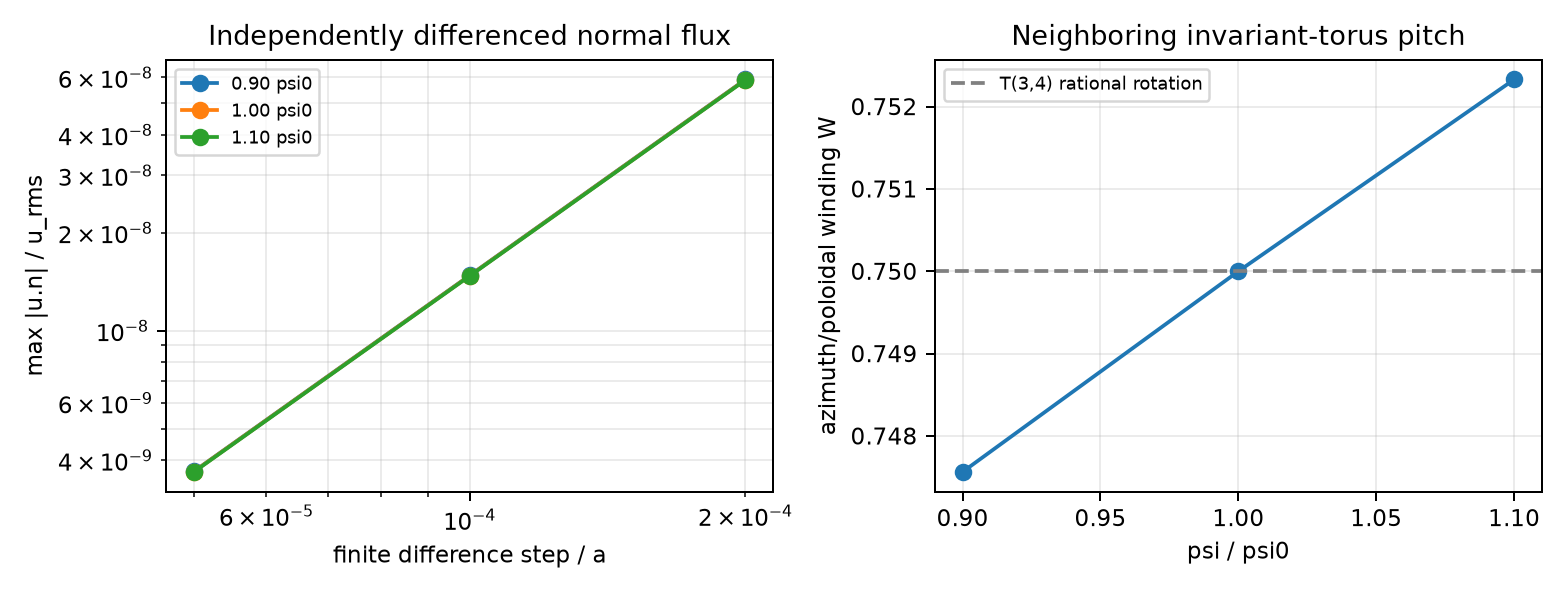
\includegraphics[width=.88\linewidth]{flux_and_shear.png}\caption{FD-normal flux convergence (left) and invariant-torus winding shear (right). Winding shear is kinematic and is not a 3D Euler instability growth rate.}\end{figure}
\section*{4. Frozen parent evidence and continuation semantics}
Parent v0.2.0 gate statuses were loaded from byte-hashed files, checked against its original gate ledger and source-seal hash, and \emph{not recomputed or rewritten}. The failed steady constant-normal-radius tube (T5 FAIL) and constant rotation of neighbor lines (T6 FAIL) remain historical results. A v0.2.1 S6 FAIL specifically rejects \emph{the psi-level torus as a knotted-core construction}; it is not a proof that no other knotted material surface could exist.
\section*{5. New gate ledger}
\small\begin{longtable}{p{.07\linewidth}p{.14\linewidth}p{.69\linewidth}}\toprule
Gate & Status & Qualification \\\midrule
S0 & PASS & Are frozen parent v0.2.0 hashes and FAIL/UNRESOLVED status immutable? \\
S1 & PASS & Does fresh integration reproduce frozen T(3,4) reference line? \\
S2 & PASS & Do explicit closed regular psi-level contours occur at three frozen levels? \\
S3 & PASS & Does the original T(3,4) line sit on the reconstructed psi-level torus? \\
S4 & PASS & Are u and omega tangent to every regular psi-level surface? \\
S5 & PASS & Are these invariant level-set boundaries standard unknotted tori of revolution? \\
S6 & FAIL & Does the psi-level solid torus itself have a T(3,4)-knotted CORE? \\
S7 & FAIL & Does a finite interval of invariant psi levels share identical 3:4 line closure? \\
S8 & PASS & Are invariant level contours numerically converged and regular? \\
S9 & UNRESOLVED & Does v0.2.1 demonstrate an isolated finite T(3,4) vortex core stable in 3D Euler? \\
S10 & UNRESOLVED & Has native C++ FP64 v1.0.7 certification independently occurred? \\
S11 & UNRESOLVED & Can local shear/deformation establish dynamical instability without perturbed Euler? \\
\bottomrule\end{longtable}\normalsize
\section*{6. Remaining scientific blockers}
A complete falsifier of general finite-core vortex-tube persistence must construct a localized finite-vorticity field, a nonaxisymmetric material boundary with independently checked knot type, and a \emph{coupled 3D incompressible Euler perturbation/pressure evolution}. Register perturbations and grid resolutions in advance; monitor div($u$), energy, helicity, knot/link invariants, tube flux, boundary clearance and error convergence for at least ten core periods. None of these certifications was executed in v0.2.1. This is an analytical/numerical \texttt{REFERENCE\_ONLY} package, not an official v1.0.7 FREEZE/CERTIFY instance.
\textbf{Conclusion.} Smooth stationary Hicks $\psi$-tori \emph{do} exist and are material/vorticity-tangent. They are unknotted ordinary tori of revolution. A $T(3,4)$ trajectory on such a surface does not supply a stable isolated $T(3,4)$ vortex-tube core. General finite-core existence and time-dependent stability remain \textbf{UNRESOLVED}.
\section*{References}
W. M. Hicks, \emph{Researches in Vortex Motion III} (1899), \href{https://doi.org/10.1098/rsta.1899.0002}{doi:10.1098/rsta.1899.0002}. A063 v0.2.0 local archival evidence, byte-bound to v0.2.1 in \texttt{baseline/}.
\end{document}
